\newpage
\chapter{Model Synchronization}
\hypertarget{sec:synch}
\genHeader

At this stage, you have successfully created a trio of rules that can transform a \moslTggCode{Box} with any number of \moslTggCode{Partitions} and
\moslTggCode{Cards} into a \moslTggCode{Dictionary} with an unlimited number of \moslTggCode{Entrys} (or vice versa). 

Now suppose you wanted to make a minor change to one of your current instances, such as adding a single new card or entry into one of your instances. 
Could you modify the instance models and simply run the transformation again to keep the target and sources consistent? 

The current \filename{src.xmi} file (\Cref{fig:ea_extended_fwd_src_xmi}) has a partition with an index of three which, when transformed, correctly produces a target dictionary with all four entries. 
What would happen if we attempted to transform this dictionary back into the same learning box, with all four partitions?

\begin{stepbystep}

\item Copy and paste \filename{fwd.trg.xmi}, renaming it as \texttt{bwd.src.xmi}.\footnote{Feel free to either delete or rename the original \texttt{bwd.src.xmi} for later reference.}

\item Run \texttt{LearningBoxToDictionaryIntegrationTrafo.java} and inspect the resulting \texttt{bwd.trg.xmi}
(\Cref{eclipse:missingP3}). 
Unfortunately, the newest \texttt{part\-it\-ion\-3} is missing!
\end{stepbystep}

\begin{figure}[htbp]
\begin{center}
  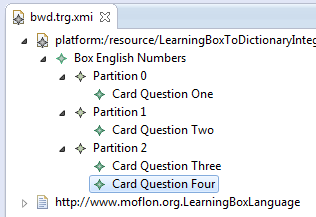
\includegraphics[width=0.5\textwidth]{../../org.moflon.doc.handbook.04_tripleGraphTransformations/7_synchronization/sImages/eclipse_missingPartition}
  \caption{We lose information if the original box has more than 3 partitions}
  \label{eclipse:missingP3}
\end{center}
\end{figure}

If you think about this for a moment it should be clear that our TGG-based backward transformation can only \emph{create} a box with exactly three partitions.
Why doesn't it try to apply \texttt{AllOtherPartitionsRule} you might be thinking?
Well, given only the target model it is simply unclear how often this rule should be applied:  Once? Twice? A hundred times?
We could of course integrate user interaction to decide, but for a TGG of realistic size this would get pretty messy pretty soon. 

When going from the source to the target model, this information (how many partitions exist) is simply discarded and lost. 
So how can we prevent this information loss when we need to update our models in the future? Luckily, eMoflon can take care of this for you as it provides a \emph{synchronization} mode to support incremental updates.

Let's change our source model by adding a new \moslTggCode{Card} to \texttt{Partition3} and see if the partition still exists after synchronizing to and from the resulting \moslTggCode{Dictionary} model.

\begin{stepbystep}
\item Make sure your \filename{fwd.src.xmi} model is in the \enquote{extended} version depicted in \Cref{fig:ea_extended_fwd_src_xmi}, and that you have a fresh triple of corresponding \filename{fwd.corr.xmi} and \filename{fwd.trg.xmi} created via the forward batch transformation.

\item Our synchronisation algorithm requires an explicit \emph{delta}\define{Delta}, a representation of the exact changes that are to be propagated.
Although this can be extracted from different versions of a model, this is not as easy as it sounds.
To make matters worse, \enquote{delta recognition} is also often not unique, \idest, there are many possible deltas for the same pair of old and new models.

As we are more interested in the actual synchronisation than in change recognition or \enquote{diffing}, we require the exact delta, which can come from anywhere in actual applications, including being programmed as a hard coded change operation in some kind of synchroniser GUI.

To play around with a TGG, however, we provide a simple \menuPath{Delta Editor,}\define{Delta Editor} which behaves very much like the standard EMF model editor, but records all the changes you make and persists them as a delta model, which we understand.

To open the delta editor, right-click on \filename{fwd.trg.xmi} and choose \menuPath{Open With/Delta Editor}.

\item Let's try a simple attribute change:  As \texttt{Entry four:vier} was created from a card in the third partition, its default level is beginner (remember we assume easy cards have wondered further into the box).
Well we think this is wrong so let's change the level to \texttt{master}.
Perform this change directly with the \menuPath{Delta Editor} as if it were the standard EMF model editor (compare with \Cref{fig:trgDelta}).
Save the editor and close it.
Take a look at the created \filename{trg.delta.xmi} and inspect it.
Although we do not (yet) have a fancy visualisation for delta models, it should be pretty easy to see how your change has been represented as a data structure.
Finally, note that \filename{trg.xmi} has \emph{not} been changed yet, \idest, the synchroniser will do this when trying to propagate your changes.
This is important to understand as handling conflicts (work in progress, planned for a release in the far, far away future) might imply a compromise, \idest, not all your changes might be accepted or possible.

\begin{figure}[htbp]
\begin{center}
  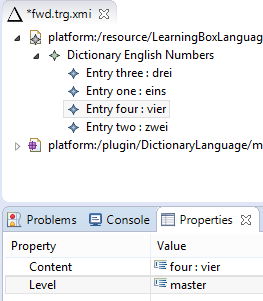
\includegraphics[width=0.37\textwidth]{../../org.moflon.doc.handbook.04_tripleGraphTransformations/7_synchronization/sImages/trgDelta}
  \caption{Change the level of an entry}
  \label{fig:trgDelta}
\end{center}
\end{figure}

\item To backward propagate your changes, open
\filename{Learning\-Box\-Language\-To\-Dictionary\-Language\-Sync.java}, our generated stub for model synchronisation.
Our stubs are optimized for this handbook so you do not have to change a thing.
It's all plain and simple Java though, so you should be able to understand
how our API is being used.
The section where you can adjust and make changes is:
\begin{lstlisting}[language=Java]
// Adjust values as required
String delta = "instances/fwd.trg.delta.xmi";
String corr  = "instances/fwd.corr.xmi";
BiConsumer<...> synchronizer = helper::syncBackward;
\end{lstlisting}

These values all fit our current change (the created delta file, the relevant correspondence model, and we want to synchronise backwards), so we're ready to go.
Hit \menuPath{Run} and see what happens!
If everything went well, \texttt{Card question:four} should have been relocated to \texttt{partition0} to fit its corrected difficulty level.
The great thing is \texttt{partition3} is now empty, \emph{and has been retained}.
Not that the protocol has been updated, and that \filename{trg.xmi} not contains these changes.
\end{stepbystep}

Remember this is all academic software and especially the delta editor is rather new and very buggy.
Feel free to try out all kinds of deltas and if you think you've found a bug, please send us an email at \emoflonMail and we'll be happy to fix it (or reply with a \enquote{back in your face!} if it's not one and \emph{you} just got confused).
